

\part{Introduction et Présentation générale}

\setcounter{section}{0}

\section{Problématiques}



Aujourd’hui de nombreuses personnes souhaitent se lancer dans l’entreprenariat, cependant le premier pas peut être difficile à faire. En effet, pour des personnes non-initiées
le monde de l’entreprise semble complexe et dangereux. C’est dans l’optique d’aider ces
personnes à estimer leur capacité à faire des choix que nous avons eu l’idée de développer un serious game sur le thème de l'entreprise. Pour ceux qui ne savent pas ce qu'est un serious game, il s'agit d'un jeu qui a pour objectif d'instruire de façon ludique tout en s'approchant le plus possible de la réalité, un petit peu à la façon d'une simulation. Nous avons ainsi établi les problématiques suivantes :
Comment approcher virtuellement l’environnement propre aux entreprises ?
De quelle manière peut-on rendre pertinentes les conséquences des choix de l’utilisateur ?



\section{Objectifs}



Dans le but de répondre à ces problématiques nous nous sommes fixés un certain
nombre d’objectifs :



\begin{enumerate}
\item[•] Modéliser une start up dont les choix de l’utilisateur déterminerons la
progression de son entreprise.
\item[•] Approcher au plus près la réalité, en se basant sur un maximum de chiffres, d’études et
de théories reconnues.
\item[•] Ancrer la structure de l’entreprise dans un univers économique où interagissent différents
acteurs.
\item[•] Modéliser l’impact des choix de l’utilisateur (management), en se basant sur des données
économiques.
\item[•] Développer une interface graphique utilisateur/machine ergonomique et intuitive.\\
\end{enumerate}
De même nous avons quelle que piste de refléxion pour faire évoluer le projet dans le temps comme par exemple:
\begin{enumerate}
\item[•] Intégrer les facteurs humains tels que le bonheur, le stress, etc... En effet ces facteurs
possèdent un impact significatif sur la productivité.
\item[•] Modéliser de nouvelles branches de développement que ce soit pour le joueur avec la gestion du marketing, ou encore en modélisant des risques extérieurs à l'entreprise telque des évenements aléatoires comme des catastrophes naturelles ou encore des greves de ses partenaires économiques.
\item formation des ind
\end{enumerate}



\clearpage



\section{Cadre applicatif}



Après avoir effectué des recherches bibliographiques sur le sujet, nous nous sommes consacrés cette année au développement d'une application répondant à nos objectifs ci-dessus. Notre but est donc de faire un serious game le plus fidèle possible à la réalité.\\
Dans le but d’être le plus réaliste possible, nous allons utiliser des théories provenant des domaines que sont le management, l’économie et l’analyse prédictive. La partie management nous permettra de proposer un panel de choix suffisamment large à l’utilisateur. La partie économie nous donnera les moyens mathématiques d’inscrire notre entreprise virtuel dans un monde approchant la réalité, par l'implémentation de modèles se rapportant au monde économique.
En essayant de faire figurer les différents acteurs. Enfin, la partie portant sur l’analyse
prédictive, servira à déterminer l’évolution de nos variables en fonction des choix.

















\clearpage























\clearpage



\part{Le développement de l'application}



\setcounter{section}{0}



Dans cette section nous allons vous exposer comment fonctionne notre application. Ainsi que comment l'installer et la faire fonctionner.



\section{Manuel d'utilisation:}



\subsection{Comment installer:}



\subsection{Comment bien débuter:}



Une fois le jeu lancer, vous vous retrouver devant l'écran principal. Plusieur choix son à votre disposition:



\begin{enumerate}
	\item[•] Commencer une partie, se bouton vous emmenera vers une page de création de partie, dans laquelle vous choisirer les conditions initiales de votre entreprise (capital, nombre d'employé et autre).
	\item[•] Charger une partie, vous permettr comme son nom l'indique de charger une partie existante.
	\item[•] Quitter, vous ferra fermer le jeu.
\end{enumerate}

Normalement si vous lancer le jeu pour la première fois, il ne devrait pas y avoir de sauvegarde. Il vous faudra donc créer une nouvelle partie.  Pour cela cliquer sur le bouton "Commencer une partie", une nouvelle page apparait vous demandant votre nom. Ce nom sera aussi celui de votre sauvegarde.\\

Une fois cela fait vous voici dans le menu principal, il vous permet d'acceder à différentes fenêtres:



\begin{enumerate}
    \item[•] Accueil.
    \item[•] Ressources Humaines.
    \item[•] Recherche et Développement.
    \item[•] Production.
    \item[•] Finances.
    \item[•] Ventes.
    \item[•] Options.
    \item[•] Aides. 
\end{enumerate}



\clearpage



Pour gagner de l'argent, il vous faut un produit pour par la suite vendre. Vous commencer la partie avec plusieurs produits. Allez ensuite dans la page "Production", puis dans l'onglet "Produire". Ici vous avez acces à vos différents produits, selectionné s'en un. La fenêtre se modifie et vous affiche un tableau à deux colonnes, la première représente votre stock et la seconde la demande en composant du projet que vous avez selectionné.\\

S'il vous manque des composants, allé dans l'onglet "Approvisionnement" (juste au dessus de "Produire") et approvisionné vous en composants, pour pouvoir débuté la production de votre produit. Lorsque les composants que vous avez commandé seront arrivés, vous recevrez une notification, qui s'affichera dans l'onglet "Accueil". En attendant vous pouvez finir votre tour ou commencé la recherche d'un nouveau produit.
\\

Pour cela rendez vous dans l'onglet "Ressources Humaines" pour engager une personne qui sera responsable de la recherche liée à votre produit. Une fois dans l'onglet "Ressources Humaines" cliquez sur "Recruter" qui vous permettra d'embaucher un employé. \\

Choisissez celui qui possede les meilleurs statistiques pour la tache que vous voulez lui attribuer. Ici nous voulons un individu qui a un score en compétense en recherche élevé en principal, et des scores en coopération et management pas trop mauvais. Car même si ces deux derniers facteurs impactent moins la vitesse de recherche ils ne sont pas non plus négligeable.\\

Voila vous avez recruté votre premier salarié. Maintenant vous devez lui attribuez une tache. Pour cela rendez vous dans l'onglet "Recherche et développement, cliquer sur "Ajouter un projet" qui créer un nouveau projet. Une fois cela fait, vous devez choisir les employés que vous voulez attribuer à ce projet. Noté que tant que vous n'avez pas donné de nom et cliqué sur le bouton "Ajouter le projet", vous pouvez changer d'avis et modifié la liste des employés ajoutés. Simplement en cliquant sur la case de l'employé, une fois décidé donné un nom à votre projet et cliqué sur "Ajouter le projet".\\

Vous receverez une notification à chaque fois que votre poduit change de stade de développement. Les notifications s'afficheront dans l'onglet "Accueil", cliqué dessus pour voir se qu'il vous demande, la plupart du temps il s'agira seulement d'approuver le prochain stade de développement.
\\

Une fois vos composants reçus, allez dans l'onglet "Production" puis "Produire" vous pouvez si vous avez tous les composants nécessaires lancer la production de ce produit. Lorsque le produit est fin prèt il peut être mis en vente via l'onglet "Vente", selectionné votre produit, puis cliqué sur "Mettre en vente" pour le vendre, il y aura une notification si vous ne remplissez pas toutes les conditions, par exemple vous ne disposé pas d'assez de se produit en stock.\\

De plus dans l'onglet finance vous pouvez gérer vos prêts et observer le bilan des dépenses de votre entreprise.\\

Maintenant vous savez comment embauché un salarié, créer un nouveau produit, et gérer son développement jusqu'à sa vente. Il reste encore quelques fonctionnalités que vous pouvez utiliser comme la possibilité de faire des prèts ou améliorer un produit déja existant. Mais ces fonctionnalités sont assez simple d'utilisation et reprennent les mêmes idées de bases que celle déja expliqué préalablement.



\subsection{Actions possibles}



Dans cette partie, vous retrouverez la liste de l'ensembles des actions sur l'application. Elles sont triées par rapport à leurs branches de l'entreprise ou leurs fonctionnalités dans le programme.\\



\subsubsection*{Sur le menu principal}



Créer une partie : Cliquez sur le bouton "Commencer une partie" puis insérez un pseudo, un nom ou un prénom dans la zone de saisie puis cliquer sur le bouton "Continuer".\\

Charger une partie : Cliquez sur le bouton "Charger une partie" puis sur la liste à gauche, cliquez sur la sauvegarde que vous souhaitez charger s'il existe. Ensuite cliquez sur le bouton "Chargez" sur le panneau de droite, en dessous des informations de la sauvegarde sélectionnée.\\

Quitter le jeu : Cliquez sur le bouton "Quitter".\\



\subsubsection*{Dans le jeu}



Les actions ci-dessous peuvent être réalisées à n'importe où dans l'application.\\

Changer de branche de l'entreprise : Cliquez sur l'un des 6 premiers boutons de la barre de navigation fixé sur la gauche de la fenêtre. Vous serez rediriger vers la branche en question.\\

Accéder au menu Option : Cliquez sur le 7ème bouton en partant du haut de la barre navigation ou bien pressez sur la touche ECHAP de votre clavier.\\

Accéder à l'aide : Cliquez sur le bouton le plus en bas de la barre de navigation pour accéder à l'aide de la page sur laquelle vous vous trouvez actuellement.\\



\subsubsection*{Accueil}



Passez à la semaine suivante : Cliquez sur le bouton "Tour suivant".\\



\subsubsection*{Ressources Humaines}



Les actions ci-dessous sont réalisées à partir de la branche Ressources Humaines de l'application.\\

Recruter un candidat : Cliquez sur le bouton recruter sur le bas du panneau de gauche. Puis sélectionner un candidat dont vous voulez voir les caractéristiques ou bien recruter. Ensuite cliquez sur le bouton "Recruter" du panneau de droite pour le recruter.\\

Voir les caractéristiques d'un employé : Cliquez sur l'un des employés de la liste des employés à la droite de la fenêtre.\\

Licencier un employé : Cliquez sur l'employé que vous souhaiter licencier dans la liste des employés. Puis cliquez sur le bouton "Licencier".\\



\subsubsection*{Recherche \& Développement}



Les actions ci-dessous sont réalisées à partir de la branche Recherhce \& Développement de l'application.\\

Voir la liste des projets : Cliquez sur l'onglet "Projets". \\

Créer un projet: Cliquez sur le bouton "Ajouter un projet". Ensuite cliquez sur des employés de la liste de gauche que vous souhaiter ajouter au projet et donnez un nom à ce dernier. Vous pouvez retirer des employés en cliquant sur ceux de la liste de droite. Cliquez enfin sur le bouton "Ajouter le projet". \\

Voir les caractéristiques d'un projet : Cliquez sur un projet dans la liste à droite de fenêtre s'il en existe. \\

Voir les participants d'un projet : Cliquez sur un projet dans la liste à droite de fenêtre s'il en existe puis cliquez sur l'onglet "Participants". \\

Ajouter des participants à un projet : Cliquez sur le projet auquel vous voulez ajouter des participants dans la liste à droite de fenêtre s'il en existe puis cliquez sur l'onglet "Participants". Cliquez ensuite sur le bouton "Ajoutez des participants". Sélectionnez des employés à ajouter dans la liste de droite puis cliquez sur le bouton "Ajouter au projet". Vous pouvez retirer des employés en cliquant sur ceux de la liste de droite.\\

Supprimer un projet : Cliquez sur le projet que vous souhaitez supprimer puis cliquez sur l'onglet "Supprimer". \\

Voir la liste des produits : Cliquez sur l'onglet "Produits". \\

Voir les caractéristiques d'un produit : Cliquez sur un produit de la liste des produits. \\

Améliorer un produit : Cliquez sur un produit de la liste des produits puis cliquez sur l'onglet "Améliorer". Ensuite sélectionnez les employés qui vont améliorer le produit en cliquant dessus. \\



\subsubsection*{Production}



Les actions ci-dessous sont réalisées à partir de la branche Production de l'application.\\

Voir le tableau de bord : Cliquez sur l'onglet "Tableau de bord". \\

S'approvisioner en matériaux : Cliquez sur l'onglet "Approvisionnement". Puis sélectionner le matériaux à acheter. Choissisez le founisseur en le cliquant dessus. Entrez la quantité de matériaux à acheter puis cliquez sur "Suivant" et ensuite "Passez la commande". \\

Lancer la production d'un produit : Cliquez sur l'onglet "Produire". Puis sélectionner le produit à produire. Entrez la quantité de produit à commander si vous le pouvez sinon allez vous approvisionner en matériaux nécessaires. Ensuite sélectionner un machine en cliquant dessus. Ensuite s'il n'y a aucun utilisateur sur la machine, sélectionner un employé à mettre sur la machine en le cliquant dessus. Enfin appuyez sur le bouton "Passez la commande". \\

Afficher la liste des stocks : Cliquez sur l'onglet "Stocks". \\

Afficher la liste des machines : Cliquez sur l'onglet "Machines". \\

Acheter une machine : Cliquez sur le bouton "Acheter une machine" au dessus de la liste des machines. Puis cliquez sur le bouton "Acheter" de la machine dont vous souhaitez acheter. \\

Ajouter/retirez un employé à une machine : Cliquez sur le bouton respectif sur une machine de la liste des machines. Si vous souhaitez en ajouter, sélectionner l'employé à mettre sur la machine en cliquant dessus. \\



\subsubsection*{Finances}



Les actions ci-dessous sont réalisées à partir de la branche Finances de l'application.\\

Voir le résumé de la branche Finance : Après avoir cliquez sur l'onglet "Prêt", cliquez sur l'onglet "Résumé". \\

Voir la liste des prêts : Après avoir cliquez sur l'onglet "Prêt", cliquez sur l'onglet "Liste des prêts". \\

Contracter un prêt : Après avoir cliquez sur l'onglet "Prêt", cliquez sur l'onglet "Contracter un prêt". Choisissez le type de prêt en cliquant sur le bouton "Court", "Moyen" ou "Long". Ensuite entrez la durée du prêt et le montant puis cliquez sur le bouton "Générez". Attention, le montant maximum du prêt est généré seulement après avoir cliquez sur le bouton "Générez" et dépend de la durée entrée. Ensuite cilquez sur le bouton "Ok". \\

Voir le bilan financier : Cliquez sur l'onglet "Bilan". \\

Voir le compte de résultat : Cliquez sur l'onglet "Compte de résultat". \\

Voir la Macroéconomie : Cliquez sur l'onglet "Macroéconomie". \\



\subsubsection*{Ventes}



Les actions ci-dessous sont réalisées à partir de la branche Ventes de l'application.\\

Voir le tableau de bord : Cliquez sur l'onglet "Tableau de bord". \\

Afficher la liste des produits : Cliquez sur l'onglet "Produit". \\

Mettre en vente un produit : Après avoir cliquez sur l'onglet "Produit", cliquez sur un produit à mettre en vente puis cliquez sur l'onglet "Mettre en vente". Ensuite, si vous avez de ce produit en stock, entrez la quantité de produit à vendre et le prix de ce dernier puis cliquez sur le bouton "Mettre en vente". \\



\subsubsection*{Option}



Les actions ci-dessous sont réalisées à partir de la fenêtre Option.\\

Sauvegarder : Cliquez sur le bouton "Sauvegarder". \\

Retourner au menu principal : Cliquez sur le bouton "Retourner au menu principal". \\

Quittez le jeu : Cliquez sur le bouton "Quittez". \\

Supprimer la sauvegarde : Cliquez sur le bouton "Supprimez la sauvegarde"













\part{Explication}



\setcounter{section}{0}



\section{La Partie Design}

La fenêtre est réalisée à l'aide de Pygame, la bibliothèque graphique de Python. Elle permet notamment l'affichage de divers formes, d'images ou bien encore de textes. De cette librairie ont été crée des "widgets", comme par exemple des boutons, des barres de défilement ou des zones de saisies de textes. Ces dernier nous permettant ainsi de voir et d'intéragir avec les différentes variables du jeu. \\
Les couleurs choisies pour l'application sont dîtes "flat" et donne un aspect moderne et sérieux à ce dernier.


\section{Les Menus}



\subsubsection*{La Sauvegarde}



Pour la partie qui sauvegarde(save) et charge(load) nous utilisons l’extension pickles de python. A l’aide de cette extension nous sauvegardons toutes les variables importantes (qui sont pour la plupart des objets) tels que les employés ou encore les différents produits.  Nous avons passé quelque temps à chercher un outil python qui nous permettrait de sauvegarder et de charger efficacement et sans trop de difficulté nos différentes variables. Pickles était donc parfait pour cette tâche car la fonction de sauvegarde et de chargement ne prennent que quelque ligne ( une dizaine pour les deux) de plus pickles permet de sauvegarder sous n’importe quelle extension que se soit du .txt ou encore .sav. 











\section{La Partie Ressources Humaines:}



La partie des ressources humaines permet d’avoir un aperçu des différents aspects stratégiques liés aux employés. 



\subsection{Les individus:}



Les «individus» désignent les différents employés de l’entreprise et les candidats potentiels pour le recrutement. Ils ont entre 23 et 60 ans. Nous les créons en python sous forme d’objet avec différentes caractéristiques. Parmi celles-ci, on retrouve : \\



\begin{itemize}
    \item[•] L’Expérience en R\&D. Un individu peut avoir entre 0 et 37 ans d’expérience en R\&D. On génère donc l’expérience d’un individu en fonction de son âge: un travailleur de 23 ne peut pas avoir d’expérience mais un travailleur de 53 ans peut avoir entre 0 et 20 ans d’expérience. Cette expérience va déterminer une partie de la valeur des compétences relatives à la R\&D.\\


    \item[•] L’Expérience dans la Start-up. Cette dernière nous permet de connaitre le nombre de semaines qu’a passée l’individu dans la Start-up.\\


    \item[•] L’Expérience en Production. Elle désigne le nombre de temps qu’un utilisateur a passé à utiliser les machines de production de l’entreprise. Elle est donc à 0 pour tout nouvel employé.\\


    \item[•] Les compétences en R\&D. Elles sont trois: la compétence de groupe qui désigne la capacité de l’individu à travailler en groupe, la compétence de recherche qui désigne la capacité de l’individu à faire avancer la recherche activement et la compétence de direction qui désigne la capacité de l’individu à diriger une équipe. Ces compétences sont représentées sous la forme d’une valeur entre 1 et 10. Elles tirent 50\% de leur valeur de l’expérience en R\&D (soit 5 points de compétence sur 10 au maximum). Ainsi, un individu qui a 37 ans d’expérience en R\&D se voit automatiquement attribué 5 points de compétence de recherche, de par son expérience. Finalement, entre 1 et 5 points supplémentaires sont attribués aléatoirement. Ils représentent le «talent» de l’individu.\\


    \item[•] La compétence de production. Cette expérience modélise l’efficacité d’un employé sur une machine de production. 80\% de sa valeur (soit 8 points sur 10) est calculée à partir de l’expérience de production à l’aide d’une formule. Cette formule a l’allure d’une racine carrée: elle augmente rapidement au début puis se stabilise. Cela représente la rapide prise en main d’une machine par un employé puis la difficulté à progresser significativement sur l’emploi d’une machine. La formule est faite de telle manière qu’au bout de 2 semaines, l’employé voit sa compétence augmentée d’un point et il faut 3 ans pour atteindre les 8 points. Finalement, entre 1 et 2 points sont attribués aléatoirement. Ils représentent le «talent» de l’individu. 
\end{itemize}



\subsection{Le Recrutement:}



Lorsque l’on commence une partie, l’entreprise ne possède aucun employé. Il y a par contre 5 candidats pour le recrutement. Tous les mois, 5 nouveaux candidats prennent leur place. Cela modélise le renouvellement des candidats avec relativement peu de demande pour un emploi en start-up.



\subsection{Les Salaires:}



Pour parler de salaire on parlera de salaire brut. On se servira également du site de l’Apec pour évaluer les salaires. Les employés sont actuellement tous recrutés en CDI.

En R\&D, nous partons du principe que l’entreprise embauche des ingénieurs. Ainsi, pour des individus bac+5 travaillant dans la conception, recherche en électronique dans une entreprise de 1 à  19 salariés en Ile de France en CDI, on obtient les salaires moyens pour les différentes durée d'expériences. Par exemple, pour moins de 4 ans d'expérience pro, le salaire moyen est de 30.6k\euro{}/an brut. Soit 2550\euro{}/mois brut. 



les paliers d'expériences que nous prendrons sont :



\begin{itemize}
    \item[] 0-3 ans : 2550\euro{}
    \item[] 4-5 ans : 2975\euro{}
    \item[] 6-8 ans : 2975\euro{}
    \item[] 9-16 ans : 3483\euro{}
    \item[] 17-33 ans : 3858\euro{}
    \item[] 34$+$ ans : 4025\euro{}
\end{itemize}



Nous allons aussi appliquer ces salaires aux employés en production car ils sont très similaires à ceux de production sur le site de l’Apec.



\subsubsection*{Pour aller plus loin:}



On pourra par la suite diversifier les rôles, les niveaux d’études, la nature des contrats, adapter les salaires à  la taille de l’entreprise. Voire même laisser la possibilité à  l’utilisateur de modifier les salaires pour rajouter une autre dimension stratégique. On pourra aussi lisser les salaires pour que les paliers soit par années (plutôt que mr.X ait le même salaire pendant 3 ans quand il est débutant). Tous ces paramètres permettront de diversifier les salaires.



\subsection{Le Coût de l’emploi:}



C’est un des coûts principaux de l’entreprise, il s’agit de la somme du total des salaires nets, des charges sociales salariales, des charges patronales et des charges indirects (dans notre cas, le coût des locaux).\\



\begin{itemize}
    \item[] salaire net $=$ salaire brut $*$ 0,78

    \item[] charges sociales salariales $=$ salaire brut $*$ 0,22

    \item[] charges patronales $=$ salaire brut $*$ 0,42\\
\end{itemize}



Cout total des employés $=$ salaires nets $+$ charges sociales salariales $+$ charges patronales $+$ charges indirectes



\subsubsection*{Pour aller plus loin:}



On pourra par la suite implémenter le CICE (Crédit d'impôt pour la compétitivité et l'emploi) et la loi Fillon qui réduisent les coûts de l’emploi. Nous avons déjà effectué des recherches sur le sujet mais faute de temps, elle ne sont pas encore implémentée.



\subsection{Coût des locaux:}



Après recherche sur meilleursagents.com, nous avons trouvés qu’en moyenne, le coût des locaux est de 23,5\euro{} le mètre carré sur la bordure extérieure de Paris. De plus, après recherches, il faut 15$m^{2}$ de surface pour 2 personnes puis $5*n+5 m^{2}$ pour $n$ employés.



\subsection{Pour aller plus loin:}



\subsubsection*{Les Formations:}



Les permettent aux employés d’améliorer leurs compétences mais génèrent des coûts pour l’entreprise. C’est un autre élément stratégique de la gestion des ressources humaines. Cette partie n’est pas encore implémentée mais certaines de fonctions qui s’y rattachent sont déjà prêtes.



\subsubsection*{Le Bonheur:}



Cette partie servirait à rajouter un aspect stratégique sur le fait de veiller au bien-être des employés sous peine de départs prématurés. Cette partie n’est pas encore implémentée car très complexe. Elle reste par contre dans les améliorations pertinentes que pourront être ajoutée au programme.



\subsubsection*{Les Licenciements:}


Les licenciements ne sont actuellement pas pénalisants mais cela fait partie des éléments prioritaires à être ajoutés dans le futur du projet. En se servant bien évidement de recherches sur le droit du travail et les lois qui entourent le licenciement en France.







\section{La Partie Recherche et Développement}





La section Recherche et Développement (R\&D) d'une entreprise a pour objectif de créer, de concevoir des produits innovants, que ce soit à partir d'un concept ou bien d'un produit déjà existant. Dans une première partie, nous détaillerons nos différents choix d'implémentation pour modéliser le processus de création d'un tout nouveau produit (partie recherche). Dans une seconde partie, nous montrerons comment l'utilisateur peut améliorer un produit (partie développement).
\paragraph{Hypothèse :} Dans le but de rendre possible une modélisation de cette section de l'entreprise, nous avons posé l'hypothèse suivante : \textit{On considère que nos chercheurs ne sont jamais à court d'idées. Ainsi seuls les temps relatifs à l'élaboration du projet, au développement technique et aux tests de validation pourront être différents selon les projets}.

\subsection{Innovation}
Pour notre modélisation nous nous sommes basé sur un modèle simplifié des étapes du processus de développement de produits et nous en avons tiré les étapes suivante : 
\begin{enumerate}
\item[•] Analyse du marché et création d'un concept;
\item[•] Mise en forme d'un premier prototype;
\item[•] Création d'un prototype;
\item[•] Tests de validation du produit;
\item[•] Déposition du brevet.
\end{enumerate}
\subsubsection{Concept}
\noindent
Au début de tout processus de création, le produit n'est qu'une idée, un concept, qu'il va falloir développer pour pouvoir en faire un produit commercialisable. Cet "état premier du produit" est donc modélisé par l'objet \textbf{Concept}. Ce dernier possède deux paramètres : 
	\begin{enumerate}
		\item[•] \texttt{Concept.appreciation} : L'appétence des populations* (liste de listes);
		\item[•] \texttt{Concept.cible} : La population cible $\in \left\{ "Jeunes", "Actifs", "Seniors"\right\}.$.\\ 
	\end{enumerate}
\noindent
* \textit{: Pour avoir de amples informations quant aux populations, nous vous invitons à vous référer à la partie} Environnement.\\\\
\noindent
Détaillons à présent les fonctions associées à cet objet :
\begin{enumerate}
	\item[•] \textbf{sondage() :} Cette fonction a pour but de créer une appréciation sur le concept pour chaque population. Appréciation définie aléatoirement par la fonction \texttt{aleaLoiNormale()} (\textit{cf} Outils). L'appréciation se présente comme une liste d'éléments dont la forme est explicitée ci-après :
	\begin{center}
		\texttt{[(résultat, score), Population.nom]}	
	\end{center}
\end{enumerate}
\noindent
\texttt{résultat} : une chaine de caractères qui indiquera à l'utilisateur le résultat du sondage. Il existe 4 types de résultats différents : "indifférents", "intéressés", "enthousiastes" ou "très enthousiastes".\\
\texttt{score} : un nombre flottant créé aléatoirement par la fonction \texttt{aleaLoiNormale()} :\\
\begin{center}
\texttt{score}$=$\texttt{aleaLoiNormale(esperance$=50$,ecart\_type$=16.6$)}
\end{center}
C'est ce nombre qui détermine le résultat précédent :\\
Soient $x$ le score déterminé aléatoirement et $y$ le résultat. On définit la fonction $f$ avec $f(x)=y$ telle que : \\\\
$
f : \left\{ 
\begin{array}{r c l}
\mathbb{R}_{+} &\to  &\{"indifferents";"interesses";"enthousiastes";"tres\ enthousiastes"\} \\\\
x\in [0;50] &\to &"indifferents"\\
x\in ]50;75] &\to &"interesses"\\
x\in ]75;90] &\to &"enthousiastes"\\
x\in ]90;100] &\to &"tres\ enthousiastes"
\end{array}
\right.
$\\\\
\texttt{Population.nom} : une chaine de caractères qui renseigne le nom de la population associée à cette appréciation.
\begin{enumerate}
	\item[•] \textbf{ciblage() :} Cette fonction prend en paramètre le choix de l'utilisateur quant à la population qu'il souhaite cibler avec son concept. Puis met à jour le paramètre \texttt{Concept.cible}.
	\item[•] \textbf{effetMarketing() :} Lorsqu'un produit cible une certaine partie de la population, celle-ci est plus attirée de part l'effet marketing. C'est ce que cette fonction modélise : elle augmente le \texttt{score} du concept pour la population cible ce qui peut modifier le \texttt{resultat} de celle-ci. Le calcul du bonus se fait à l'aide de la fonction \texttt{aleaLoiNormale()} :
	\begin{center}
		\texttt{bonus}$=$\texttt{aleaLoiNormale(esperance$=5$, ecart\_type$=1.6$)}
	\end{center}
\end{enumerate}

A la fin de la phase 1 de la création d'un produit, le \texttt{Concept}, doté d'une appréciation et d'une population cible devient un \texttt{Prototype}.

  
\subsubsection{Prototype}

En effet, un concept, une idée de produit ne devient pas un produit fini et prêt à la vente du jour au lendemain. C'est pourquoi, nous avons modélisé le produit en développement par la classe \texttt{Prototype}. Cette classe va nous permettre de définir les matériaux, les opérations et l'utilité de notre futur produit, tout en conservant l'appréciation et la population cible de l'objet \texttt{Concept}\\

\noindent
	L'objet \textbf{Prototype} est caractérisé par :
	\begin{enumerate}
		\item[•] \texttt{Prototype.appreciation} : L'appétence des populations (liste de listes);
		\item[•] \texttt{Prototype.cible} : La population cible $\in \left\{ "Jeunes", "Actifs", "Seniors"\right\}.$;
		\item[•] \texttt{Prototype.materiaux} : La liste des matériaux qui le composent (liste de Materiau.nom);
		\item[•] \texttt{Prototype.operations} : La liste des opérations nécessaires à sa fabrication (liste d'Operation.nom);
		\item[•] \texttt{Prototype.cout} : Son coût de fabrication (nombre décimal).
	\end{enumerate}
\noindent
Détaillons à présent les fonctions associées à cet objet :

\begin{enumerate}
	\item[•] \textbf{creaMater() :} Génère la liste des matériaux nécessaires à la création du prototype.
	\item[•] \textbf{creaOpera() :} Génère la liste des opérations nécessaires à la création du prototype.
	\item[•] \textbf{creaCout() :} Calcule le coût de fabrication du prototype en fonction du prix des matériaux.
	\item[•] \textbf{develop() :} Cette fonction permet d'exécuter les trois fonctions précédentes en une seule fonction.
	\item[•] \textbf{apprToUti() :} Converti l'appréciation du prototype en une utilité. Nous définissons l'utilité suivant un concept de la microéconomie : la fonction d'utilité. Celle-ci mesure en quelque sorte l'appétence des utilisateurs par rapport à un produit donné. La conversion de l'appréciation en utilité suit la fonction suivante : \\ \\
Soit $x$ une valeur de la liste \texttt{Prototype.appreciation} pour une population donnée et $y$ la valeur de l'utilité correspondante dans la liste \texttt{Produit.utilite} : 	
	\begin{align*}
		y =\frac{1}{125}\cdot x^{2}
	\end{align*}
Comme nous le verrons dans la partie \texttt{Ventes} de notre projet, l'utilité fait partie du coefficient déterminant la part d'acheteurs dans une population donnée. Notons que l'utilité est proportionnelle au nombre d'acheteurs. Pour indication, la fonction ci-dessus est construite de la sorte qu'un score d'appréciation de $100$ donne un score d'utilité de $80$.
% A développer 
\end{enumerate}

\noindent
Une fois que l'on a converti l'appréciation en utilité, nous pouvons enfin créer notre \texttt{Produit}. Celui va prendre en paramètres la liste des matériaux et des opérations ainsi qu'une utilité et une population cible.  


\subsubsection{Produit}

Nous arrivons ainsi à la classe \texttt{Produit}. Celle-ci représente les produits de notre entreprise. En effet l'utilisateur pourra en produire un certain nombre pour ensuite les vendre aux consommateurs. 

\noindent
	L'objet \textbf{Produit} est caractérisé par :
	\begin{enumerate}
	\item[•] \texttt{Produit.nom} : Un nom unique pour le produit, que l'on utilisera pour identifier le produit dans la liste des produits de l'utilisateur (chaine de caractères);
	\item[•] \texttt{Produit.utilite} : La liste contenant les utilités associées aux populations : "Jeunes", "Actifs" et "Seniors";
	\item[•] \texttt{Produit.cible} : La population cible $\in \left\{ "Jeunes", "Actifs", "Seniors"\right\}.$;
	\item[•] \texttt{Produit.materiaux} : La liste des matériaux qui le composent (liste de Materiau.nom);
	\item[•] \texttt{Produit.operations} : La liste des opérations nécessaires à sa fabrication (liste d'Operation.nom);
	\item[•] \texttt{Produit.prix} : Le prix de vente unitaire du produit (entier).
	\item[•] \texttt{Produit.marche} : Une variable indiquant si le produit est en vente (booléen). 
	\item[•] \texttt{Produit.age} : Le temps passé du produit sur le marché en semaine (entier)  
	\item[•] \texttt{Produit.develop} : Une variable indiquant si le produit est en développement (booléen).
	\item[•] \texttt{Produit.nbr\_ameliorations} : Le nombre d'améliorations du produit (entier). 
	\end{enumerate}
	
	En lui même, l'objet produit ne possède pas beaucoup de fonctions qui lui sont propres. En effet, nous avons juste implémenté une fonction pour pouvoir définir le prix d'un produit selon une entrée utilisateur et une fonction pour mettre à jour \texttt{Produit.age}. 
	
\subsubsection{Projet}
\noindent
	C'est l'objet \texttt{Projet} qui va modéliser un projet, et ainsi les différentes étapes de création en donnant à l'utilisateur la possibilité de faire des choix quant au développement de son produit.
	L'objet \textbf{Projet} est caractérisé par :
	\begin{enumerate}
	\item[•] \texttt{Projet.nom} : Un nom pour le projet (string).
	\item[•] \texttt{Projet.produit} : L'objet en développement. Celui-ci sera tout d'abord un Concept, un Prototype et un Produit.
	\item[•] \texttt{Projet.avancement} : C'est en quelque sorte la quantification de la progression du projet durant une phase. Cet avancement est incrémenté chaque semaine par la fonction suivante :
\begin{center}
	\textbf{avance(projets, paliers, employes)}
\end{center}
	\texttt{projets} : La liste complète des projets en cours dans l'entreprise que ce soit des objets Projet ou Ameliore (\textit{cf. La prochaine partie}) \\ \\
	\texttt{paliers} : La liste des paliers. Nous avons initialisé cette liste de la façon suivante : paliers=[80, 100, 100, 100]. Les valeurs ont été prise de telle sorte que la réalisation d'une phase de développement prennent en moyenne un temps raisonnable (~$2$-$3$ mois) \\ \\
	\texttt{employes} : La liste des employés de l'entreprise.\\
	
	Le gain d'avancement d'un projet en fonction des employés qui lui sont associé est calculé de la façon suivante : \\ \\
\noindent	
Soit $n$ le nombre d'employés du projet, on définit : $R_{i} \in \llbracket 0, 10 \rrbracket$ la compétence de recherche du $i$-ème individu, $G_{i} \in \llbracket 0, 10 \rrbracket$ la compétence de groupe et $L_{i} \in \llbracket 0, 10 \rrbracket$ la compétence de leadership avec $i \in \llbracket 0, n \rrbracket$. 
	\begin{align*}
		S_{r} &= \sum_{i=0}^{n} R_{i}\\
		m_{l} &= \underset{i \in \llbracket 0, n \rrbracket}{\sup} (L_{i}) \\
		S_{g} &= 10\cdot\left( \left\lfloor \frac{m_{l}}{8} \right\rfloor \left(m_{l}-7\right) + \frac{1}{n}\cdot \sum_{i=0}^{n} G_{i}\right) -50		
	\end{align*}
	
	Plus simplement dit, nous faisons la somme des compétences recherche des individus, et une moyenne des compétences de groupe de l'équipe de chercheurs (en ajoutant un bonus si un des chercheur possède une compétence de management supérieure ou égale à $8$). Cette moyenne représentera un pourcentage bonus ou malus de la somme $S_{r}$. En effet on considère qu'une équipe qui ne travaille pas efficacement en groupe diminue sa productivité. A contrario, un groupe sachant travailler ensemble aura un bonus sur sa productivité. Pour indication ce facteur peut aller de $-50\%$ à $+50\%$. 
	\begin{align*}
	Avancement\ total &= S_{r}+\frac{S_{g}}{100}\cdot S_{r}
	\end{align*}
	
	\item[•] \texttt{Projet.phase} : Un entier indiquant à quelle étape se situe le projet. \texttt{Projet.phase} $\in \llbracket 1, 5 \rrbracket$.
	\item[•] \texttt{Projet.attente} : Variable indiquant si le projet requiert une action de l'utilisateur (booléen).
	\item[•] \texttt{Projet.essai} : Variable indiquant si le produit a été mis à l'essai durant la phase $4$ (booléen).
	\end{enumerate}
	
\subsection{Amélioration}
Dans l'objectif de modéliser, le développement d'un produit nous avons dans un premier temps listé les différents types d'amélioration possibles :
\begin{enumerate}
	\item[•] Réduction des matériaux.
	\item[•] Réduction des opérations.
	\item[•] Augmentation de l'utilité auprès des consommateurs.
\end{enumerate}
	\noindent
Dans un second temps, nous avons créé un objet \texttt{Ameliore}, qui va modéliser le développement d'un produit. Cet objet est caractérisé par : 
\begin{enumerate}
	\item[•] \texttt{Ameliore.produit} : Le produit en cours de développement (Produit).
	\item[•] \texttt{Ameliore.avancement} : L'avancement de l'amélioration incrémentée à chaque semaine comme pour l'objet \texttt{Projet}.
	\item[•] \texttt{Ameliore.palier} : Variable définissant la valeur d'avancement à avoir pour finir l'amélioration. 
	\item[•] \texttt{Ameliore.phase} : A l'état actuel, il n'existe qu'une seule étape (ce qui justifie que le palier soit une simple valeur et non une liste). A la fin de celle-ci on passe directement à la phase $5$, pour que le projet soit considéré comme terminé.
	\item[•] \texttt{Ameliore.attente} : Variable indiquant si l'amélioration requiert une action de l'utilisateur (booléen). 
\end{enumerate}
	
La fonction principale de l'objet \texttt{Ameliore} est \textbf{update()} : cette fonction génère préalablement une variable aléatoire en utilisant la fonction \texttt{aleaLoiNormale()} : 
	\begin{center}
		\texttt{bonus}$=$\texttt{aleaLoiNormale(esperance$=50$, ecart\_type$=\sigma$)}\\
		Avec $\sigma = \frac{16}{1+Ameliore.produit.nbr\_ameliorations}$ 			\end{center}
Soit $x$ la valeur définit plus haut et $y$ le type d'amélioration, on définit la fonction $f$ avec $f(x)=y$ telle que : \\\\
$
f : \left\{ 
\begin{array}{r c l}
[0, 100] &\to  &\{"materiaux", "operations", "utilite"\} \\\\
x\in [0;34[ &\to &"materiaux"\\
x\in [34;66] &\to &"utilite"\\
x\in ]75;100] &\to &"operations"
\end{array}
\right.
$

Si le type d'amélioration est "materiaux" alors on prend un materiaux associé au produit aléatoirement et on lui retire 1 à sa quantité. On fonctionnera de la même façon pour l'amélioration de type "opérations". Quant à l'utilité nous l'augmentons de \texttt{aleaLoiNormale($10$, $1.6$)}-\texttt{produit.nbr\_amelioration}.









\section{La Partie Production et Vente}



\subsection{Création des matériaux et des opérations}



Pour la partie consernant la création des composants, ces derniers sont définis de la façon suivante: un nom, un pays distributeur, et un prix à l'unité. Pour les différents composants que nous avons sélectionnés nous avons essayé de respecter au maximum la réalité, autrement dit pour un certain composant fabriqué majoritairement en Europe et en Asie, alors dans notre application il sera importable de ces deux régions. En plus de cela nous avons essayé de rapprocher les écarts de prix pour un même produit qu’il soit importé d’un continent ou d’un autre.

Pour cela nous nous somme rendu sur diférentes plateformes de vente sur différents continents, pour ainsi suprimer l'impacte des transports car nous calculons ces couts nous même.

Pour la partie sur opération nous avons cherché à couvrir le plus large paterne de prix possible, pour proposer une grande variété de produit. De plus nous avons choisi des opérations de complexités différentes qui vont du soudage jusqu’à la vulcanisation.  Toutes les opérations sont des opérations bien réelles. Bien que leur prix soit complètement et leurs durées soient fictives nous avons essayé de respecter les échelles de prix selon leurs complexités et leurs difficultées.



\subsection{La modélisation de la carte et des transports}



Comme nous l'avons définit plutôt notre jeu tente de se rapprocher le plus fidèlement possible de la réalité. Pour la partie de recherche sur la modélisation des transports, nous avons choisit de rechercher tous les distances, les temps et les coûts de transport pour les sauvegarder dans une base de donné. L’avantage de cette méthode est que nous n’avons pas eu à modéliser à proprement parler une carte du monde ce qui à grandement simplifié le développement. Néanmoins rechercher toutes ces données pour les transports, c’est révélé plus compliqué que prévu. Les recherches, sur les temps de transport ou encore les distances entre les différente fournisseur, étaient assez rapide et simple.
\\

Contrairement aux recherches sur les coûts de transports se sont révélée un véritable calvaire car l’un des seuls moyens pour les obtenir est de faire des devis à des sociétés de transport, le problème étant qu’il faut être un professionnel( dans le sens où il faut posséder une véritable entreprise) pour pouvoir accéder à ces devis. Il nous a donc fallu arpenter l'internet à la recherche de devis rendu publique par des entreprises qui importaient ou exportaient vers les destinations qui nous intéressaient. Ces devis étant assez rare car peu d'entreprises  sont aptes à rendre publique ces chiffres sensibles. En tout cas pour les transports maritimes. Pour les transports terrestres nous nous sommes basés sur la formule suivante:

((prix d'entretient du camion + prix de l'essence au kilometre)$*$(distance en kilometre)$+$(salaire horaire d'un camionneur)$*$(distance$/$vitesse moyenne))$*$(marge transporteur)

Pour le transport entre Paris et Berlin par exemple on obtient:

(0.535€$*$800km$+$(17\euro{}$/$h)$*$(800km$/$(60km$/$h)))$*$1,3
\\

Pour simplifier les choses nous avons basé nos transport sur des conteneurs de vingt pieds(taille standard des conteneurs 20x8x8 pieds), nous avons de même négligé l’impact du poid de ces derniers dans les coûts de transport car premièrement nous ne gérons pas l’encombrement du poids dans nos entrepôts et deuxièmement nous avons tous simplement trouver aucune valeur accessible aux particulier.

Une remarque que l'on pourrait faire, est que si l'utilisateur commande un seul matériau, il devra payer le prix d'un transport via des containers (alors que si il l'importait par la poste les couts seraient peut être cent fois moins chères)


\subsection{Les fournisseurs}

Nous commençons par créer un objet que nous appellons Fournisseur. Nous débutons par lui donner un nom, puis une localisation. Les localisations sont séléctionnées depuis la liste suivante: 

\begin{enumerate}
\item[] Paris
\item[] New York
\item[] Hong kong
\item[] Berlin
\item[] Amsterdam
\end{enumerate}
Chaque fournisseur à sa propre localisation qui lui est unique. C'est à dire que pour l'instant comme nous avons six localisations différentes, nous ne pouvons avoir que six fournisseurs différents. Par la suite nous ajoutons tous les matériaux, définie dans la base de donné, que les fournisseurs peuvent vendre. Pour cela nous recherchons dans la base de donné matériaux tous les éléments qui sont fabriqués dans une certaines localisations. Par exemple si notre fournisseur est localisé à Paris, il pourra vendre tous les matériaux provenant de cet endroit. Les matériaux sont définis de la façon suivante: un nom, un pays, et un prix à l'unité.\\

%Dans cette class nous définissons aussi d'autres fonctions comme la fonction approvisionnement, qui à partir des fournisseur, de la destination, de la commande faite par l'ulisateur, et de l'argent qui lui reste sur son compte, modifie l'objet transport en ajoutant le nouveau transport à ceux déja éxistant. De plus cette fonction modifie l'objet couts en lui ajoutant les couts de transport et le cout de la commande faite par le joueur. Pour finir la fonction renvoie l'argent qui reste à l'utilisateur après sa commande.\\



\clearpage



\subsection{Les Opérations:}



Les opérations font partie des 2 composantes nécessaires à la fabrication d’un produit avec les matériaux. Elles sont déterminées au lancement d’une partie. Dans l’absolue, se ne sont pour l’instant que des éléments distincts les uns des autres et qui participe à diversifier les produits et à complexifier l’aspect stratégique du jeu. 



\subsubsection*{Pour aller plus loin:} 



On pourra par la suite lier les opérations aux matériaux nécessaires pour plus de réalisme et$/$ou de stratégie quant au choix des machines à acheter$/$utiliser.



\subsection{Les Machines:}



Les machines permettent de réaliser les opérations nécessaires à la fabrication d’un produit. Elles sont présentes physiquement dans l’entreprise, qui s’occupe elle-même de la production. On leur assigne un employé qui fera donc usage de sa compétence en production. Nous avons créé un système de commandes, elles sont chacune attribuées à une machine (qui peut réaliser toutes les opérations nécessaires à la fabrication du produit concerné) et si celle-ci a un utilisateur, la production se met en route.



\subsubsection*{Pour aller plus loin:} 



On pourra par exemple faire en sorte que plusieurs machines soient nécessaires à la fabrication d’un produit. Diversifier les prix des machines. Nous pourrons aussi sous-traiter la production (ce qui était l’idée d’origine) en passant par des usines présentes dans différents pays et avec différents coûts.



\subsection{La Fabrication d’un produit:}



Pour la production, on considère que la semaine de travail dure 5 jours et les employés travaillent 8 heures par jour. Ainsi, il y a 40 heures de travail par employé sur une semaine. Soit 2400 minutes. C’est le temps de travail qu’un employé débutant fournit par semaine.


Lors de la production, nous utilisons une formule qui traduit la compétence de l’employé travaillant sur la machine en capacité de travail. En fait, nous considérons qu’un individu avec une compétence en production élevé est plus efficace sur les machines et fournit plus de «temps de travail» par semaine. Ainsi, comparé à un employé débutant (1 ou deux points de compétence en production), un employé qui à 3 ans d’expérience soit (9 ou 10 points) en production a une capacité de production deux fois plus élevée. 

$x =$ compétence de l’utilisateur

charge de travaille$ = (300/9)*x^{2} - (300/9)*x + 2400$


Lorsqu’un produit est complètement terminé, c’est-à-dire quand les matériaux ont tous été consommés quand toutes les opérations nécessaires ont été réalisées, le produit est ajouté au stock de l’entreprise.


\subsection{Les Stocks:}


Les stocks sont les endroits où l’entreprise entrepose ses matériaux et ses produits. Ils ont une capacité de stockage et génèrent des coûts chaque mois. Actuellement, il n’y a qu’un seul stock et il se situe dans l’entreprise.


\subsubsection{Pour aller plus loin:} 

Nous pourrons créer d’autres stocks pour pouvoir gérer des matériaux et des productions à l’étranger (dans des usines étrangères par exemple). Avec les transports pour relier les différents points.


\subsection{Les ventes:}
	
Afin que l'utilisateur puisse vendre les produits qu'il a crées, nous avons dû modéliser les consommateurs. Dans notre modélisation, un consommateur n'est pas un individu mais un ménage. Pour reprendre la définition de l'INSEE (Institut national de la statistique et des études économiques) un ménage désigne l'ensemble des occupants d'un même logement sans que ces personnes soient nécessairement unies par des liens de parenté. Il se peut qu'un ménage soit composé d'une seule personne. Pour mener à bien notre modélisation nous considérerons qu'un ménage désigne une seule et unique entité économique.
	
\paragraph{Définition des ménages :} Nous avons récupéré les données démographiques de la population française. Et par catégories de population ("Jeunes", "Actifs", "Seniors") nous créons $100$ types de revenus autour de la moyenne associée à la catégorie de la population en utilisant la fonction \texttt{aleaLoiNormale()}. 
	
\paragraph{Définition du budget :} Pour définir le budget des différentes populations nous nous basons sur les données de l'INSEE quant aux revenux de la population française selon les années et les tranches d'âge. Nous avons également fait des recherches sur le budget moyen dépensé dans l'achat de produit technologique pour un ménage environ $5\%$. 
	
\paragraph{La demande :} A présent nous devons définir la demande, c'est à dire, le nombre d'acheteurs total sur une année. Nous résolvons ici la problématique du consommateur : \\
	A l'aide de l'utilité du produit, nous définissons un pourcentage de la population qui souhaite acheter le produit :
\begin{align*}
	acheteurs\ potentiels = \left\lfloor  d + u\cdot\frac{1}{1000}\right\rfloor
\end{align*}
Avec $d$ le nombre de ménages correspondant à cette population, $u$ l'utilité du produit associé à la catégorie de la population 
	Ensuite nous vérifions que la population possède le budget suffisant pour acheter le produit. \\
\noindent
Ensuite par semaine nous déterminons le nombre d'acheteurs par semaine en fonction du temps du produit passé sur le marché. Le nombre d'acheteur augmentera progressivement jusqu'à atteindre un maximum avant de diminuer progressivement jusqu'à devenir nulle.
\paragraph{L'offre :} L'offre est simplement représentée par les produits se trouvant dans le stock, \texttt{market}. Celui-ci contient l'ensemble des produits, associés à une quantité, mis sur le marché.
\paragraph{Le nombre de vente :} On définit le nombre de ventes comme la valeur  minimale entre l'offre et la demande. 
\paragraph{Le chiffre d'affaire :} On calcule le chiffre d'affaire en effectuant le produit entre le nombre de ventes et le prix du produit. On calcule la tva associée à chaque vente.








\section{La Partie Finance}



\subsection{Organisation}



La fenêtre finance a pour objectif de permettre à l’utilisateur de gérer la finance de l’entreprise, par le biais de rapports détaillés des transactions financières se déroulant au sein de celle-ci. Pour organiser celle-ci, nous avons choisi de la sectionner en différentes parties:





\begin{enumerate}
\item la page principale a pour but donner les informations sur les revenus et les dépenses effectués durant la semaine
\item le groupe de page “Contracter un prêt” permet de gérer les prêts, que ce soit en contracter, ou voir ceux actuels
\item les pages bilan et compte de résultat affichent, comme l’indique leur nom, le bilan et le compte de résultat mensuellement
\item la page macroéconomie doit contenir les tableaux sur les facteurs macroéconomiques, mais elle n’est pas encore disponible
\end{enumerate}



\subsection{Récupération et affichage des données}



La page principale a donc comme objectif d’afficher les dépenses et revenus de la semaine. Nous avons donc tout d’abord besoin de récupérer ces données. Après avoir cliquer sur le bouton “Fin du tour”, un certain nombre de fonctions vont être appelées avant de passer à la semaine suivante. Nous créons alors une liste vide qui va, en parcourant ces fonctions, récupérer les différents revenus et dépenses de la semaine. Par exemple, lorsque les fonctions simulant la vente des produits seront appelées, la liste récupérera le chiffre d’affaire de la vente. Il se va de même pour chaque dépense. \\

\begin{figure}[!htb]
\centering
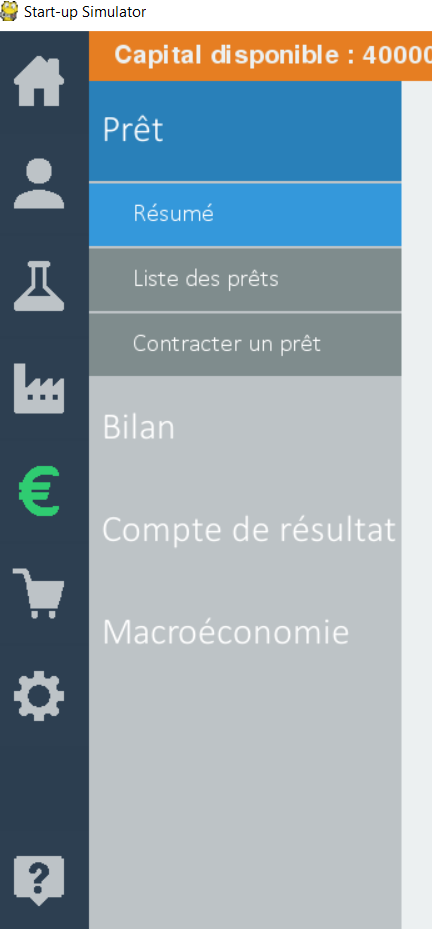
\includegraphics[scale=1]{img/menu.png}
\caption{Organisation de la section finance}
\end{figure}

Après avoir récupéré cette liste, il nous reste qu’à l’afficher sur la page principale, en différenciant les revenus et les dépenses.
Ainsi, l’utilisateur aura facilement accès aux informations financières qui se sont déroulées lors du tour de jeu.



\subsection{Bilan et compte de résultat}



En tant que serious game de gestion d’entreprise, il est primordiale que l'on respecte les bases de la comptabilité d’entreprise, que ce soit d’effectuer un bilan et un compte de résultat. \\
Traditionnellement, ceux-ci sont réalisés à la fin de chaque année. Cependant, nous avons pensé que, comme nous travaillons sur une start-up, la notion de temps peut différée. Nous voulons dire par là que les premières années sont primordiales au lancement de la start-up, et il est donc nécessaire de pouvoir accéder à un nouveau bilan et compte de résultat assez fréquemment. Nous actualisons donc ceux-ci chaque mois. De plus, vu qu’ils sont générés automatiquement grâce à nos algorithmes, la tâche de les réaliser est moindre.



\subsubsection{Bilan}



Commençons donc par le bilan. Le bilan a pour but de synthétiser ce qui est possédé par l’entreprise (l'actif), et ce dont elle dispose comme ressource (le passif).
Nous avons voulu que notre bilan reste clair, et qu’il reste à compréhension de tous. Nous ne voulons pas que l’utilisateur ait besoin d’un expert comptable ou des cours sur la comptabilité financière pour pouvoir lire notre bilan, au contraire des vrais bilans. Nous avons alors choisi d’indiquer uniquement les éléments qui nous ont semblé les plus pertinents. \\

\begin{figure}[!htb]
\centering
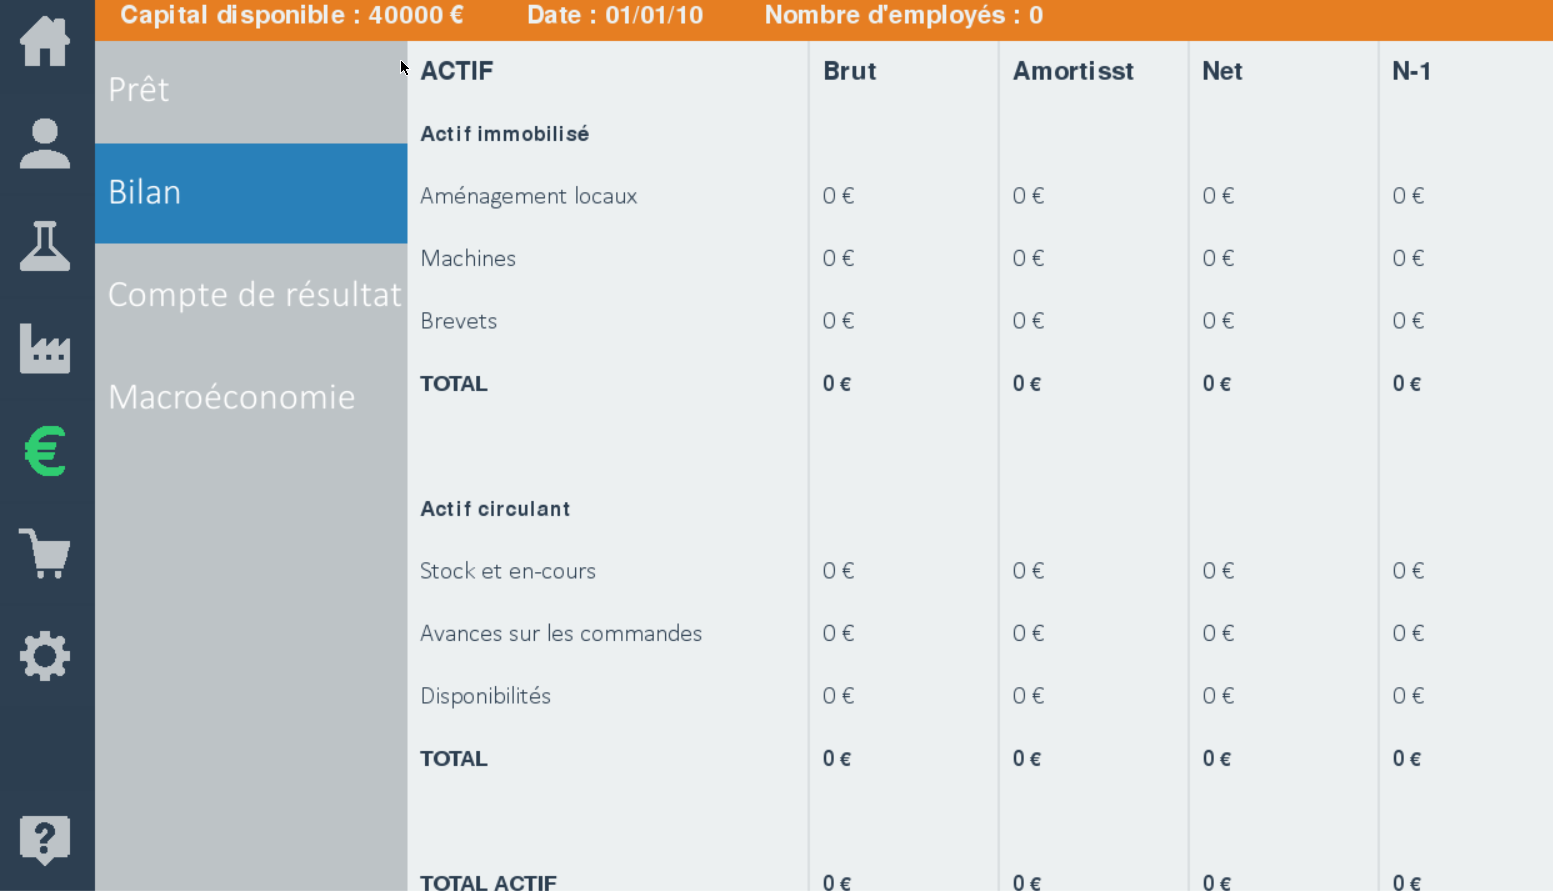
\includegraphics[scale=0.5]{img/actif.png}
\caption{Actif}
\end{figure}

\begin{figure}[!htb]
\centering
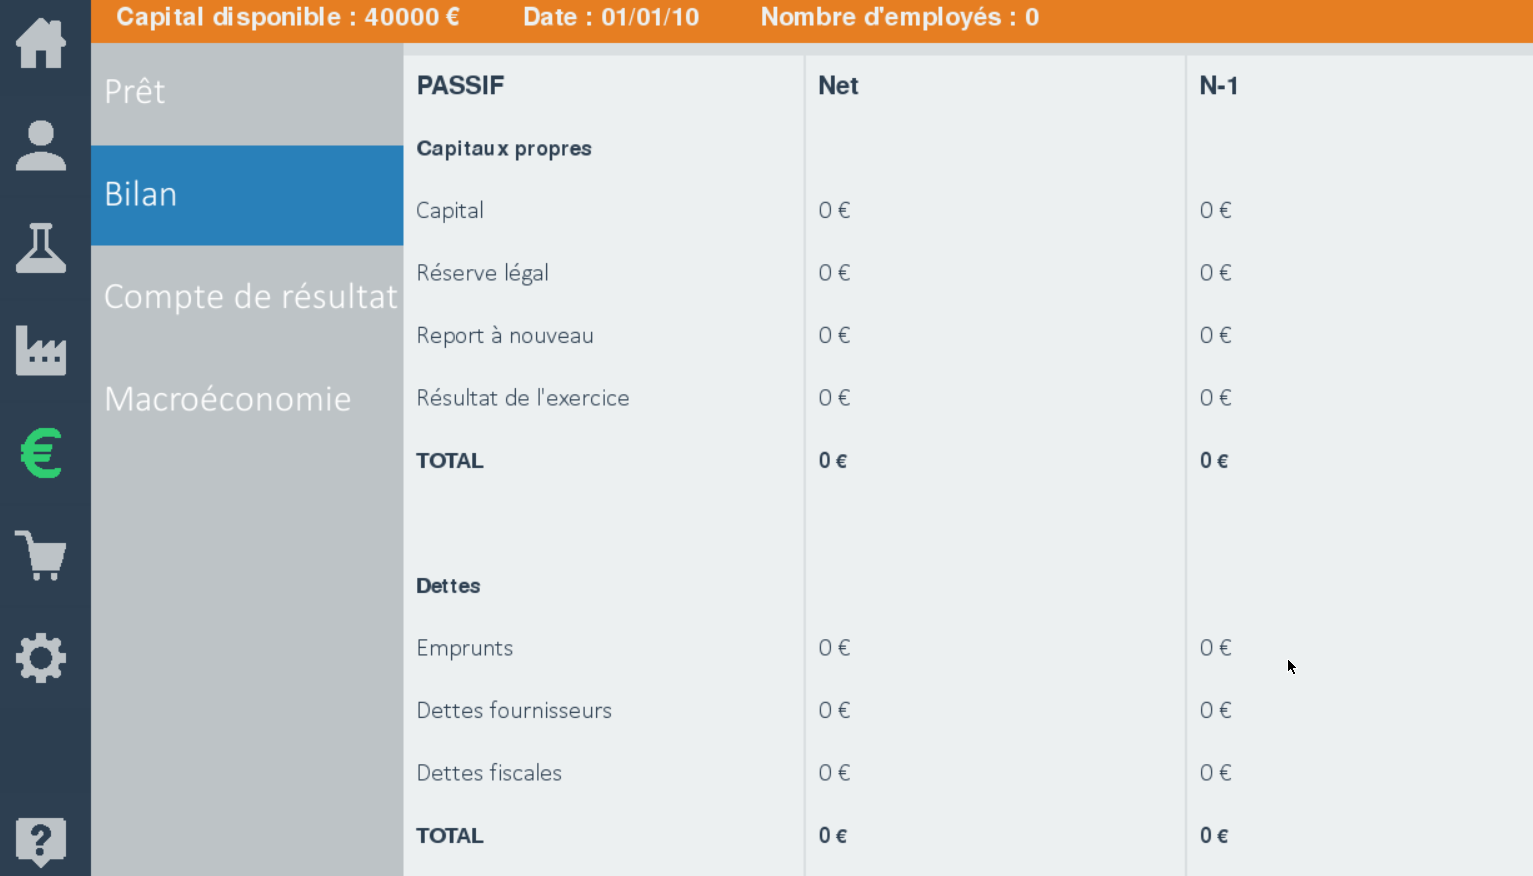
\includegraphics[scale=0.5]{img/passif.png}
\caption{Passif}
\end{figure}

Nous n’allons pas expliquer chaque élément de ce bilan, mais quelques points nécessitent des éclaircissement sur comment nous l’avons implémenter en programme.



\paragraph{Amortissement:} Tout d’abord, nous avons introduit dans le bilan la notion d’amortissement. Nous l’utilisons pour les machines. En effet, les machines n’ont pas la même valeur à l’achat que 5 années plus tard. L’amortissement nous permet ainsi de représenter plus justement la valeur des biens possédés par l'entreprise. Ainsi, chaque année, la valeur de chaque machine diminue, et cette valeur est inscrite dans la colonne 'net'. La valeur d’achat est quant à elle indiquée dans la colonne 'brut'.



\paragraph{Réserve et résultat:}La réserve légale est un compte de réserve, qui doit être égale à 10\% du capital. Ce plafond est atteint progressivement par prélèvement de 5\% du bénéfice à la fin de chaque année. Cependant, comme nous réalisons le bilan mensuellement, nos prélèvement s’élèvent à 5/12 \%. Une fois les 10\% atteints, l'obligation prend fin.



\paragraph{Report à nouveau:}Le report à nouveau est l’accumulation des résultats de l’exercice, soit les bénéfices de l’entreprise. En effet, l’entreprise ne possède pas d’actionnaires, et on ne permet donc pas de verser des dividendes.



\subsubsection{Compte de résultat}



Le compte de résultat a pour but de présenter l'ensemble des produits et des charges d'une entreprise durant un exercice comptable. Il permet ainsi d’estimer les performances réalisées par l’entreprise, et également d’en déduire le résultat de l’exercice. \\
Comme pour le bilan, nous avons voulu qu’il reste simple et claire, tout en restant cohérent. \\
\\
Dans ce compte de résultat, la valeur “production stockée” a été calculé en multipliant pour chaque produit son prix et son nombre stocké. \\
\\

\begin{figure}[!htb]
\centering
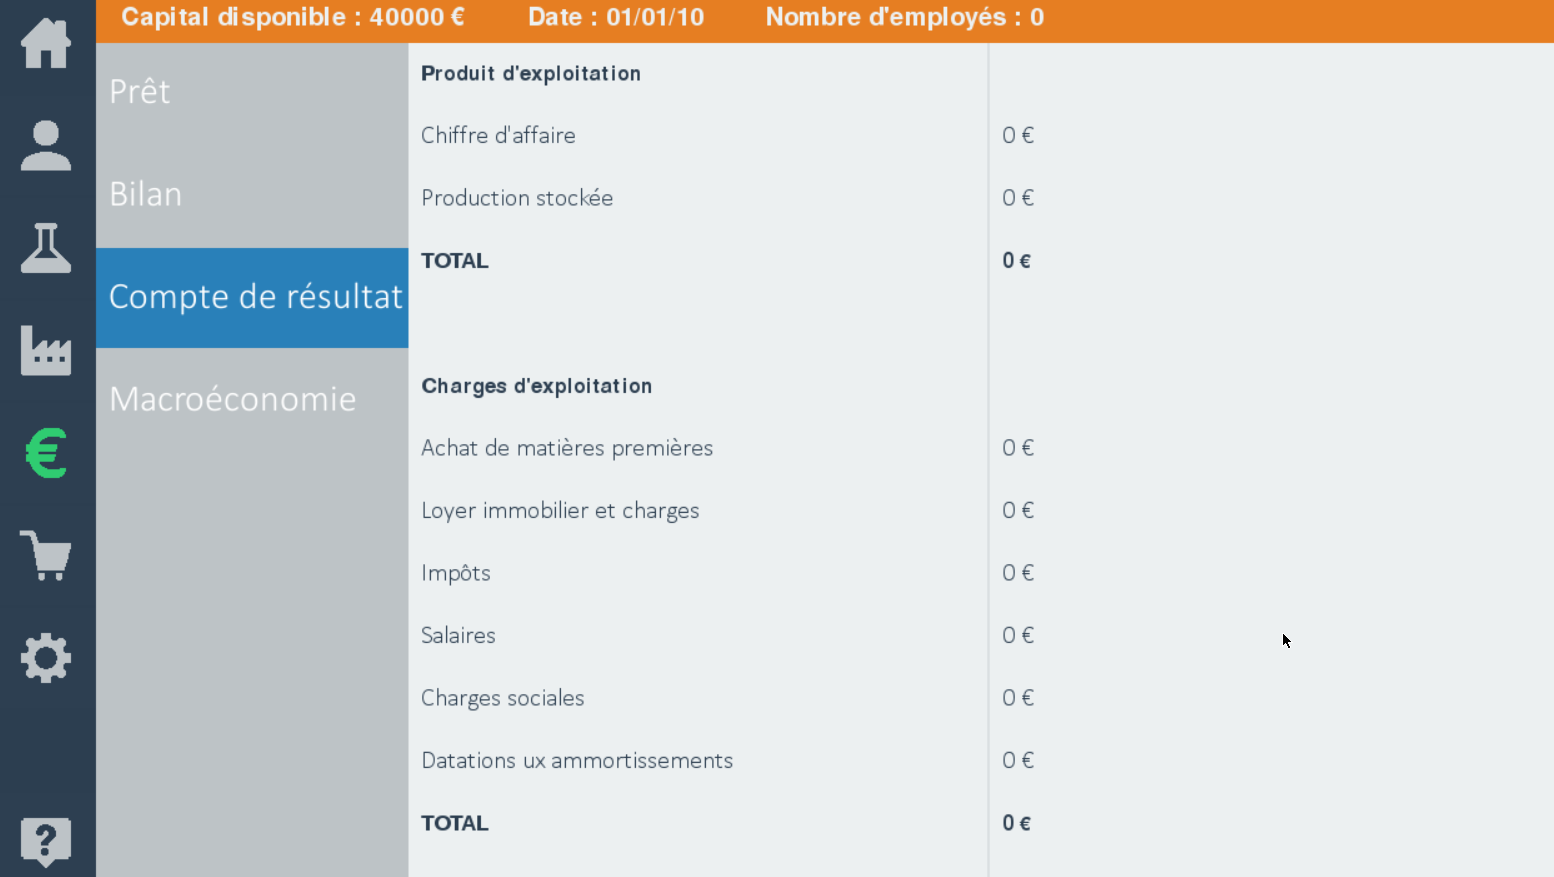
\includegraphics[scale=0.5]{img/compte.png}
\caption{Compte de résultat}
\end{figure}


\subsubsection{Taxes}



Comme vous avez pu le voir dans le bilan et le compte de résultat, nous gérons les différentes taxes que l’entreprise est amenée à payer. Plus précisément, nous prenons en compte la TVA et l'impôt sur les sociétés.



\paragraph{TVA:}



Pour chaque produit vendu, le prix de la TVA doit y être incluse. Ainsi, lorsque l’un client achète un produit, l’entreprise reçoit également le montant de la TVA. Cette valeur est stockée dans une variable qui va accumulé ces valeurs.
Par la suite, tous les 3 mois, l’entreprise doit payer ce montant à l’état. On en déduit donc cette somme au compte de l’entreprise.



\paragraph{IS:}



L'impôt sur les sociétés (IS) dépend directement du bénéfice que réalise l’entreprise. Ce bénéfice correspondant au résultat de l’exercice disponible sur le compte de résultat. Le montant de cette impôt est de 15\% du bénéfice (pour les petites entreprises comme la nôtre).  Cependant, nous effectuons le compte de résultat tous les mois. Nous effectuons donc la taxe sur les sociétés tous les mois mais à un pourcentage de 15/12 \%. La différence est existante mais négligeable.



\subsection{Contracter un prêt}



\subsubsection{Situation de l’entreprise}



Tout d’abord, il nous a paru important de pouvoir estimer la situation de l’entreprise, de pouvoir la noter. Cela nous sert alors principalement à la contraction de prêts. Cependant, dans la réalité, lorsque l’on souhaite prendre un nouveau prêt, le banquier va regarder la situation de l’entreprise pour estimer les risques possibles. Cette estimation va impacter le taux d'intérêt du prêt. Ainsi, notre estimation de l’entreprise par nos algorithmes a pour but de remplacer le regard critique du banquier. Cette partie fut donc difficile à représenter. \\
\\
Notre algorithme pour estimer la situation de l'entreprise se présente ainsi: \\
nous appelons une série de fonction qui va chacune analyser une partie de l’entreprise et qui va retourner un nombre de points, qui peut être positif ou négatif. \\
On somme les points retournés par chaque fonction, et on obtient l’estimation de l’entreprise en fonction de cette valeur. Plus le nombre de points est élevé, plus l’entreprise est en bonne situation. \\
\\
Voici les différentes fonctions incluses dans notre algorithme pour simuler l’estimation: \\



\paragraph{La croissance du chiffre d’affaire:}
Elle permet de mesurer l’évolution de l'activité de l’entreprise. \\
Pour cela, nous analysons l’évolution du chiffre d’affaire des trois derniers mois.
Cependant, une croissance élevée du chiffre d’affaire peut avoir comme résultat un endettement conséquent. Cette fonction à elle seule ne permet pas d’estimer l’entreprise. C’est pour cela que l’on ne l’estime pas à elle seule et on la cumule à d’autre fonctions.



\paragraph{La croissance des bénéfices:}
Cette indicateur est plus pertinent et complète l’évolution du chiffre d’affaire car celle-ci prend en compte également les dépenses, comme par exemple les mensualités des prêts.



\paragraph{La rentabilité:}
La rentabilité d’une entreprise est calculée en effectuant le rapport entre l’évolution des bénéfices et l’évolution du chiffre d’affaire.
Ainsi, l’entreprise a une rentabilité faible si le rapport est inférieur à 1.



\paragraph{Poids du remboursement de la dette:}
Cette évaluation est le rapport entre le chiffre d’affaire et la dette de l’entreprise.
Un ratio élevé signifie que l’endettement affecte lourdement l’activité de l’entreprise.



\paragraph{La solvabilité:}
Cette évaluation permet d’estimer si l'entreprise a la faculté de rembourser ses dettes et ses différentes ressources.
Pour cela, on compare la somme de ses actifs (sans compter la disponibilité) à ses dettes.



\subsubsection{Options du prêt}
Pour contracter un pret, plusieurs paramètres sont demandés à l’utilisateur, dont certains dépendent des autres. \\
Tout d’abord, l’utilisateur a le choix entre trois types de prêts: court, moyen et long.
Pour chacun de ses prêts, on est indique un interval de temps et également un taux d'intérêt.
Ce taux d'intérêt dépend de la situation de l’entreprise. En effet, lorsque l’on clique sur “Contracter un prêt”, on appelle une fonction pour calculer la fonction de l’entreprise. \\
Cette valeur fait varier le taux d'intérêt:


\begin{enumerate}
\item Pour le prêt à court terme: de 1,3\% à 1,7\%
\item Pour le prêt à moyen terme: de 1,2\% à 2\%
\item Pour le prêt à long terme: de 1,7\% à 2,5\%
\end{enumerate}


Pour cela, avec notre système de points, on ajoute au taux d'intérêt 0,1\% par point, avec un minimum de -0.4\% et un maximum de +0.4\%. On divise ce résultat par deux pour le prêt à court terme. \\
\\
Après avoir choisi l’option, l’utilisateur peut choisir la durée et le montant du prêt en fonction du type de prêt précédemment choisi. L’interval du montant de prêt varie en fonction également des capitaux propres de l’entreprise. On divise les capitaux par dix, puis par douze pour avoir un montant en fonction du nombre de mois. Le montant final est compris entre 0 et produit du montant calculé précédemment et le nombre de mois.\\
\\
Par la suite, on est invité à générer ce prêt, pour afficher les caractéristiques de ce prêt avant validation. On affiche le prix de l’assurance, qui correspond à 2\% du prêt.
Puis on affiche le montant de l'intérêt, qui correspond au produit du capital emprunté avec le taux d'intérêt.
Et au final, on indique la mensualité du prêt, qui correspond au montant divisé par la durée du prêt en mois.
La validation du prêt entraîne la création d’un objet “Prêt”, avec toutes les caractéristiques renseignées précédemment.



\subsubsection{Liste des prêts}
L'onglet “liste des prêt” a pour objectif, comme son nom l’indique, d’afficher tous les prêts en cours. Pour cela, on récupère une liste des prêts contenant des objets ‘Prêts’. Il est ensuite facile d’afficher, pour chacun des prêts en cours, ses caractéristiques. \\
Ainsi, pour chaque prêt, on affiche le capital emprunté, le taux d'intérêt, le total, la mensualité et ainsi que la date de contraction du prêt et sa date de fin. \\


A chaque début de mois, on prélève du compte de l’utilisateur la somme des mensualités des prêts.
Lorsque le prêt prend fin, on le supprime de la liste des prêts.



\subsection{Amélioration}
Pour compléter cette partie finance, on compte pour commencer ajouter des graphiques sur la page ‘résumé’ de la section finance. En effet, on compte ajouter trois graphiques:



\begin{enumerate}
\item un graphique circulaire dont chaque section est une dépense effectué lors de la semaine
\item un graphique affichant l’évolution des disponibilité du joueur
\item un graphique en bâton indiqué les mensualités des mois à venir
\end{enumerate}



De plus, sur la page ‘contracter un prêt’, on compte ajouter une fonction pour limiter les différentes prêts, pour qu’il ne puisse pas prendre plusieurs pret le meme mois. \\
Et enfin, il reste à compléter la page macroéconomie, où on souhaite ajouter des graphiques sur l’évolution des différentes facteurs macroéconomiques.



\part{Conclusion}



C'est avec émotion que nous achevons cette première version de notre programme. Nous avons mis beaucoup d'application dans ce projet tout au long du projet. Nous savions lorsque nous avions choisi ce sujet la complexité et la taille pharamineuse de la tâche qui nous attendait, mais nous avons pris beaucoup de plaisir à travailler sur ce projet.\\
\\
Ce projet nous a permis d'approfondir nos connaissances sur différentes notions mais également à nous initier à de nouveaux domaines, comme la comptabilité, le management ou l'économie. La complexité de ce projet nous a imposé de fournir un travail de groupe ordonné et efficace, et que chacun se spécialise dans des domaines différents.

